\documentclass{article}

% Language setting
% Replace `english' with e.g. `spanish' to change the document language
\usepackage[french]{babel}
\usepackage[fleqn]{amsmath} % Aligner les équations à gauche


% Set page size and margins
% Replace `letterpaper' with`a4paper' for UK/EU standard size
\usepackage[letterpaper,top=2cm,bottom=2cm,left=3cm,right=3cm,marginparwidth=1.75cm]{geometry}

% Useful packages

\usepackage{amsmath}
\usepackage{graphicx}
\usepackage{subcaption}

\usepackage{tikz}
\usepackage{amsmath}

\usepackage[colorlinks=true, allcolors=blue]{hyperref}

\title{TD 4 - Diffraction}
\author{IPESUP - PC }
\date{DATE}

\begin{document}
\maketitle

\section{Rappels de cours}

Le phénomène de diffraction est un phénomène qui provient du \textbf{caractère ondulatoire } de la lumière. 
Dans le cadre du programme, les situations rencontrées sont quasiment tout le temps un objet de transmittance $t(x)$ (on se limitera à des études dans une seule direction), éclairé en incidence normale par une onde plane.
La transmittance correspond comme son nom l'indique à "à quel point l'objet transmet la lumière".\\
Si on note $a_+$ et $a_-$ les amplitudes des ondes avant et après l'objet, on a $a_- = t(x) a_+$.
Attention, la transmittance est une fonction complexe et peut déphaser la lumière. 

La théorie de Fourier permet de décomposer la transmittance en une somme de fonctions harmoniques, de différentes \textbf{fréquences spatiales}. 
Ainsi, si on nomme $\xi$ la fréquence spatiale, on peut décomposer la transmittance selon la formule: $t(x) = \int_{- \infty}^{+ \infty} \hat{t}(\xi) e^{-2i \pi\xi x} dx$.
On appele $\hat{t}$ la \textbf{transformée de Fourier} de la fonction $t$.
Sa formule (non exigible) est $\hat{t}(\xi) = \int_{- \infty}^{+ \infty} t(x) e^{2i \pi \xi x} dx$.
Cette formule hideuse ne doit pas faire peur. Gardez à l'esprit qu'il s'agit de la décomposition de la fonction en une somme de sinus. 

Des calculs (vus en cours), nous ont permis de montrer qu'à la sortie de l'objet, l'onde est composée d'une superposition d'ondes planes dont le vecteur d'onde forme un angle avec l'horizontale qui est d'autant plus grand que la fréquence spatiale associée est grande.
L'angle formé entre le vecteur d'onde associé à la fréquence spatiale $\xi$ et l'horizontale suit la relation $\boldsymbol{ sin(\theta_\xi) = \lambda \xi}. $
Ainsi, si un objet contient la fréquence spatiale $\xi$, il en sort une onde plane qui forme un angle $\theta_\xi$ avec l'horizontale.
On utilise alors une lentille convergente pour former l'image de ces ondes planes. 
Il est alors très intéressant de noter qu'on obtient dans le plan focal image de la lentille ( \textbf{plan de Fourier}), une cartographie des fréquences spatiales contenues dans l'objet.


\begin{figure}[h]
  \centering
  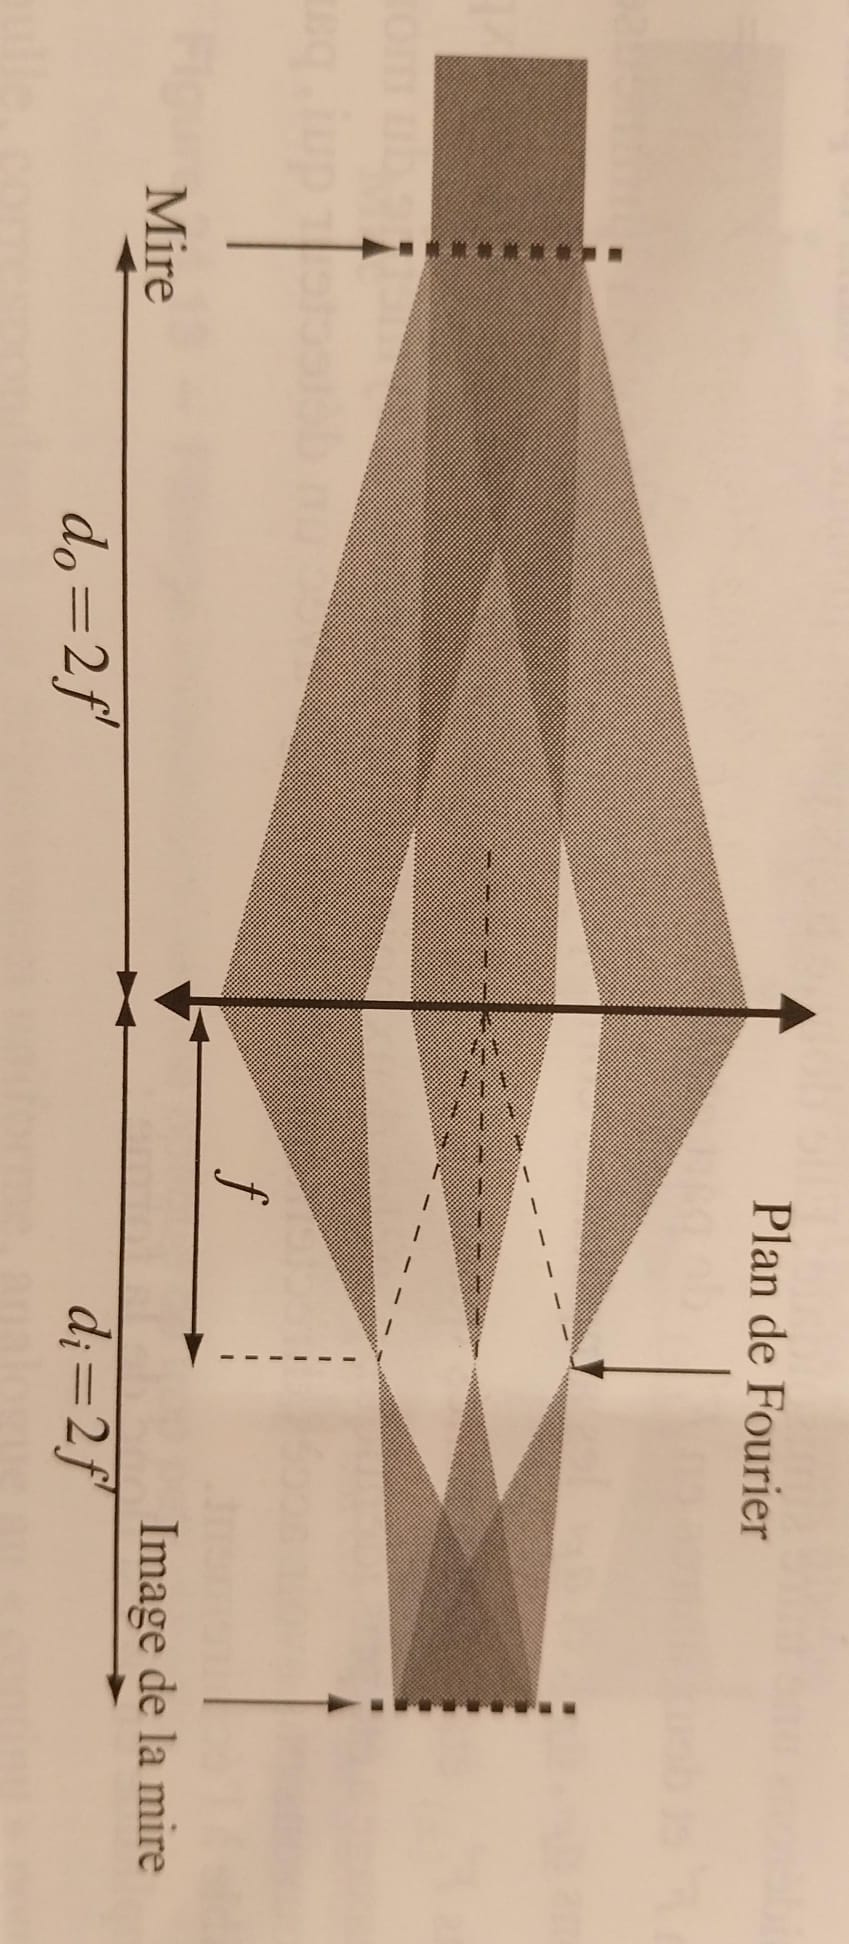
\includegraphics[width=0.3\textwidth, angle=90]{montage diffraction.jpg}
  \caption{Schéma général des figures de diffraction}
\end{figure}

On appele \textbf{objet de phase}, un objet qui a une transmittance de la forme $t(x) = e^{i \phi(x)}$ (pas de variation d'amplitude). \\
Dans le cas d'un objet infini, les fréquences spatiales apparaissent sous la forme de points. 
Si l'objet a une dimension finie (longueur $L$), ces tâches seront étendues d'une longueur caractéristique $\frac{\lambda f'}{L}$. \\


\textbf{Anecdote:} La diffraction de la lumière a été théorisée par Augustin Fresnel, un physicien français. En 1819, lors d'un concours organisé par l'Académie des sciences pour résoudre la question de la nature de la lumière, Fresnel soumit une explication mathématique détaillée de la diffraction.

L'un des juges, Siméon Denis Poisson, un fervent défenseur de la théorie corpusculaire de Newton, tenta de réfuter Fresnel en affirmant que son modèle ondulatoire menait à une prédiction absurde : si la lumière se comportait comme une onde, alors lorsqu'un disque opaque est placé devant une source lumineuse ponctuelle, un point lumineux devrait apparaître au centre de l'ombre projetée. C'était tellement contre-intuitif que Poisson pensait que cela discréditerait Fresnel.

Cependant, lorsqu'un autre membre du comité, François Arago, réalisa l'expérience en laboratoire, il observa effectivement ce point lumineux central, maintenant appelé tache de Poisson. Cette observation a validé la théorie ondulatoire et discrédité l'argument de Poisson.
\section{Filtrage d'une mire sinusoïdale}

On considère une mire sinusoïdale de période $a$ éclairée par une onde plane de longueur d'onde $\lambda$ en incidence normale. 
Cette mire est placée à une distance $d_0 = 2 f'$ d'une lentille convergente de distance focale image $f'$.
On note $F'$ le foyer image de la lentille.
L'image est observée sur un écran placé à une distance $d_i = 2f'$ de la lentille.

\begin{enumerate}
  \item Rappeler les fréquences spatiales contenues dans l'objet. En considérant que la mire a une largeur infinie, décrire l'aspect du plan de Fourier. 
  \item Quel est l'éclairement dans le plan image ? Quelles sont les fréquences spatiales de cet éclairement ? 
  \item On place un petit disque opaque de rayon $r_d$ au foyer image de la lentille. Donner une limite supérieure de $r_d$ pour que l'éclairement ne soit pas uniformément nul dans le plan image. Déterminer l'amplitude dans ce plan à un facteur de phase près. 
  \item Déterminer l'éclairement de l'image. 
  \item La largeur de la mire est en réalité finie et de hauteur $h$. Donner le rayon minimal du disque placé en $F'$ pour que la fréquence spatiale nulle soit filtrée. 
  
\end{enumerate}

\section{Principe de la strioscopie}
Dans l'exercice précédent, on garde le même dispositif mais on remplace la mire sinusoïdale par un objet de phase constitué d'une lame à faces parallèles d'épaisseur $e=0,10$ mm et d'indice optique moyen $n_0$. 
Cet objet présente des défauts, et comporte des fluctuations d'indice $\delta n$ non uniformes de l'ordre de $10^{-4}$ sur une échelle de longueur de l'ordre de $a = 1,0 $ mm. 
\begin{enumerate}
  \item Ecrire la valeur de la transmittance de la lame et la simplifier en considérant $\delta n << n_0$.
  \item Commenter l'allure du plan de Fourier avec et sans les défauts d'indice. 
  \item Décrire qualitativement l'éclairement de l'image. Peut-on voir les défauts d'indice ? 
  \item On place un petit disque opaque au centre du foyer image de la lentille, quelles sont les conséquences en terme d'éclairement ? 
\end{enumerate}


\section{Réseau de phase sinusoïdal}

On considère le même montage que dans les deux exercices précédents, mais avec pour objet une lame d'épaisseur $e_0$ dont l'indice de réfraction varie selon la loi $n(x) = n_0 + n_1 \cos \left( \frac{2\pi x}{a} \right)$.
\begin{enumerate}
  \item Ecrire la valeur de la transmittance de la lame. Proposer une décomposition en superposition de fonctions harmoniques sans chercher à calculer les coefficients. 
  \item Décrire l'aspect dans le plan de Fourier en supposant la largeur de la lame grande devant $a$. 
  \item On suppose qu'on a $\frac{n_1 e_0}{\lambda_0} <<1. $ Proposer une expression approchée de la fréquence fondamentale et de son opposée dans la transformée de Fourier. Dans la suite, on ne prendra en compte que cette fréquence fondamentale, expliquer ce choix. 
  \item Donner une expression approchée de la transmittance de la lame.
  \item En supposant la largeur de la lame $L$ grande devant $a$, déterminer l'aspect du plan de Fourier, puis celui du plan image. 
  \item Proposer une modification du montage pour améliorer le contraste de l'image. 
\end{enumerate} 
\section{Transformée de Fourier}

Déterminer les fréquences spatiales contenues dans une fente de largeur $a$ grâce à la transformée de Fourier. 


\end{document}

